Another change induced by pruning inputs is the occurrence of new
internal events that were not observed in the original log.
New events present multiple possibilities for where
we should inject the subsequent input. Consider the following case:
if $i_2$ and $i_3$ are internal events observed
during replay that are both in the same equivalence class as a single event $i_1$ from the
original run, we could inject the subsequent input after $i_2$ or after $i_3$.

% TODO: figure this figure out
%\begin{wrapfigure}{c}{1.3\linewidth}
%  \centering
%  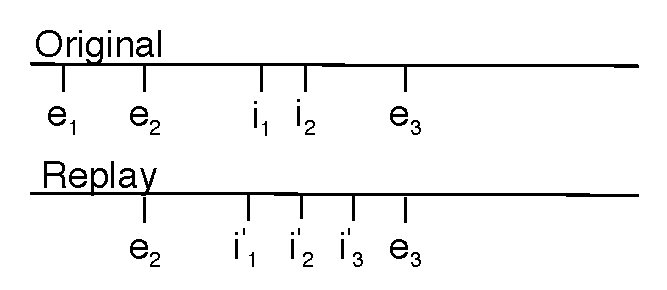
\includegraphics[width=\linewidth,height=0.8in]{../diagrams/state_machines/event_sequence.pdf}
%\end{wrapfigure}

In the general case it is always possible to construct two state machines that lead
to differing outcomes: one that only leads to the invariant violation when
we inject the next input
\emph{before} a new internal event, and another only when we inject \emph{after} a new internal
event. In other words, to be guaranteed to traverse any existing suffix that leads
to the invariant violation, we must recursively branch, trying both
possibilities for every new internal event. This implies an exponential number of
possibilities to be explored in the worst case.\footnote{
In our system, exponential search over these possibilities is not a practical option.
The heuristic our system uses when waiting for expected internal
events is to proceed normally if there are new internal events,
always injecting the next input when its last expected predecessor
either occurs or times out.}

If we assume a model of the control software's behavior, we can potentially
avoid exponential blowup.

\noindent{\bf Problem statement.} Given a predicate $\Phi(a, b)$ which for a pair of events $a$, $b$ 
(either external or internal), internal events $I$, external event $E$ we want to produce a schedule $\tau$ such that all $e\in E$ and $i\in
I$ are in $\tau$ such that:

If $a, b \in \tau$ and $a, b\in \tau_l$ then $a \rightarrow b$ ($a$ happens before $b$) in $\tau$ if and only if $a
\rightarrow b$ in $\tau_l$. This just says that $\tau$ follows the causal order in the log.

For all $a\rightarrow b\in \tau$ $\Phi(a, b)$ is true. The later is used to encode our heuristics. Assume that $\Phi$ is
well behaved with respect to events in $\tau_l$.

Two ideas for obtaining $\Phi$:

\noindent{\bf Extrapolate from complete model.} There was a paper in PLDI~\cite{vericon} that
wrote their own controller and model checked its entire state space. We could issue queries on their
state machine to compute $\Phi$, and then extrapolate $\Phi$ for other controllers assuming they are sufficiently similar.

\noindent{\bf Infer partial models using Synoptic.} We still want to maintain the constraint that we cannot modify the control software.
Even with that constraint though, we could infer a partial model of the control software by observing its behavior across many executions.
We might use Synoptic~\cite{beschastnikh2011leveraging} to achieve this.
